% ============================================================================
% main.tex — Artigo para submissão arXiv (padrão acadêmico, módulos LaTeX)
% Cada seção é um módulo \input; compila em um único PDF.
% Compilação: pdflatex main && bibtex main && pdflatex main && pdflatex main
% ============================================================================
\documentclass[11pt,letterpaper]{article}

\usepackage[T1]{fontenc}
\usepackage[utf8]{inputenc}
\usepackage[margin=1in]{geometry}
\usepackage{amsmath,amssymb}
\usepackage{booktabs}
\usepackage{array}
\usepackage{graphicx}
\usepackage{xcolor}
\usepackage{tikz}
\usetikzlibrary{arrows.meta,positioning,shapes.geometric,fit,backgrounds}
\usepackage[round,numbers]{natbib}
\bibliographystyle{abbrvnat}
\usepackage[colorlinks=true,linkcolor=blue,citecolor=blue,urlcolor=blue]{hyperref}
\usepackage{caption}
\captionsetup{font=small,labelfont=bf}
\emergencystretch=1.5em

\definecolor{cororo}{RGB}{46,116,181}
\definecolor{corverde}{RGB}{34,139,34}
\definecolor{corcinza}{RGB}{120,120,120}
\definecolor{coramarelo}{RGB}{238,180,34}
\definecolor{corvermelho}{RGB}{214,40,40}

\title{\bfseries Free LLMs in Olympic Mathematics:\\ Multi-Agent Orchestration, Cross-Validated Benchmarking, and an Architecture X-Ray\\
\large (OpenCode Ecosystem Core, evolutionary cycles R497--R500)}

\author{Marcelo Claro\\
\small OpenCode Ecosystem Core --- Autonomous Auditable Research\\
\small Preprint for arXiv submission (not peer-reviewed)}
\date{September 2026}

\begin{document}

\maketitle

\begin{abstract}
\noindent We study mathematical reasoning of \emph{free, real} large language
models (LLMs) on canonical International Mathematical Olympiad (IMO)
problems under explicit multi-agent orchestration. Across evolutionary cycles
R497--R500 of the OpenCode Ecosystem Core, we (i) curated an academic
landscape (25 sources, including \texttt{deepmind/acme}); (ii) built a
\emph{deep} diagnostics pipeline enforced by a real-execution contract;
(iii) replaced a leaking IMO harness with a deterministic anti-leak solver;
(iv) benchmarked five free models (mimo-v2.5, big-pickle, nemotron-3,
muse-spark-1.2/1.3) under raw (C0), context (C1) and 16-stage MASWOS
reasoning-scaffold (C2) conditions; and (v) implemented automatic
task$\rightarrow$model routing driven by the empirical curation (R500).
After a host restart, we ran a \emph{cross-validated} benchmark of
9 problems $\times$ 3 models. Results: the MASWOS scaffold raised first-trial
accuracy from 0\% to 100\% among models that solved at all; the single-problem
ranking of R499 (mimo 0.987 $>$ big-pickle 0.923 $>$ nemotron 0.709) does
\emph{not} survive cross-validation --- the corrected rates are mimmo 4/9
(0.44, 95\% CI [0.14, 0.79]), big-pickle 1/9 (0.11, [0.00, 0.48]) and nemotron
1/9 (0.11, [0.00, 0.48]). Paired McNemar tests are non-significant at
$n=9$; Cohen's $\kappa$ between mimo and big-pickle is $-0.216$ (they solve
different problem types). A previously hypothesized host-state explanation
for big-pickle's empty outputs is \emph{refuted}: after host restart the
model still fails (1/9). The muse-spark models exhibit ``fake reasoning''
(announce verification, deliver no answer). We report confidence intervals,
paired tests, agreement statistics, per-model latency distributions, complete
flows and an architecture x-ray (layers C0--C5). All 15 cited references have
actively validated DOIs (HTTP 200 via \texttt{doi.org}).
\end{abstract}

\noindent\textbf{Keywords:} large language models; mathematical reasoning;
multi-agent systems; cross-validation; benchmarking; IMO; uncertainty quantification.

% ============================================================================
% 00-introducao.tex — Introduction (module 1/5)
% ============================================================================
\section{Introduction}
\label{sec:intro}

Large language models (LLMs) have transformed reasoning in natural language
and mathematics. Chain-of-Thought prompting elicits intermediate reasoning
steps \citep{wei_cot}; reflective agents retry after failure
\citep{shinn_reflexion}; tool-augmented agents interleave reasoning and
action \citep{yao_react}. In formal mathematics, LeanDojo couples LLMs to a
proof assistant \citep{yang_leandojo}, and AlphaGeometry attained silver-medal
level on IMO geometry \citep{alpha_geometry}. Multi-agent frameworks such as
AutoGen \citep{wu_autogen} and MetaGPT \citep{hong_metagpt} propose program-
mable collaboration between agents. Meanwhile, standard mathematical
benchmarks --- MATH \citep{hendrycks_math}, GSM8K \citep{cobbe_gsm8k}, MMLU
\citep{hendrycks_mmlu} --- are typically evaluated on paid frontier models,
with a single trial per item and without reporting sampling uncertainty.
Recent critique \citep{schaeffer_mirage} warns that apparent capabilities may
be artifacts of discontinuous metrics; compute-optimal scaling laws
\citep{hoffmann_chinchilla} and code-trained models \citep{chen_codex}
further complicate simple narratives. Techniques that elicit latent
predictions \citep{ryoo_eliciting} extend the toolbox.

Three gaps motivate our study. \emph{First}, free-tier LLMs --- the only
option for many researchers --- are rarely benchmarked on genuine olympiad
problems with auditable pipelines. \emph{Second}, benchmarking methodology is
fragile: a single problem and a single trial cannot estimate a real accuracy
rate; confidence intervals, paired tests and cross-validation are the norm in
other fields but uncommon in LLM reports. \emph{Third}, multi-agent
orchestration effects (delegation, scaffolding, verification) are conflated
with raw model capability.

\textbf{Research question.} How can free, real LLMs be orchestrated, through an
auditable multi-agent architecture, to reason rigorously on IMO problems, and
how can the empirical evidence --- including uncertainty and limitations --- be
reported honestly?

\textbf{Contributions.}
\begin{enumerate}
  \item An auditable benchmark pipeline (R498--R499): deep diagnostics
  contract, deterministic anti-leak solver replacing a leaking harness, and a
  16-stage MASWOS reasoning scaffold (C2).
  \item Empirical ranking of five free models under scaffold conditions
  (R499) followed by a \emph{cross-validated} 9-problem $\times$ 3-model
  benchmark after a host restart (R503), with Clopper--Pearson 95\%
  confidence intervals, paired McNemar tests, Cohen's $\kappa$ and latency
  distributions.
  \item Automatic task$\rightarrow$model routing (R500) driven by empirical
  curation.
  \item A full architecture x-ray (layers C0--C5) identifying which
  components mattered, and the refutation of a host-state hypothesis.
\end{enumerate}

The remainder of this paper: \S\ref{sec:methods} methodology;
\S\ref{sec:results} results; \S\ref{sec:discussion} discussion (including
the x-ray); \S\ref{sec:conclusion} conclusion.
% ============================================================================
% 01-metodologia.tex — Methods (module 2/5) com fluxograma da validação cruzada
% ============================================================================
\section{Methods}
\label{sec:methods}

\subsection{System under test}
\label{sec:system}
All experiments ran inside the OpenCode Ecosystem Core, a multi-agent
ecosystem with 206 catalog agents, an A2A Blackboard, a metacognitive bus
(MetaBus), a Trust Engine and a strict SDD/TDD policy. The orchestrator
(MarceloClaro) executes the cycle Perceive$\rightarrow$Specify$\rightarrow$
Delegate$\rightarrow$Execute$\rightarrow$Verify$\rightarrow$Reflect. External
LLMs are invoked through the \texttt{opencode run} CLI as real subprocesses;
no simulation or mocked completion is used (Section~\ref{sec:anti-overclaim}).

\subsection{Corpus}
\label{sec:corpus}
We use a canonical IMO-AnswerBench sample (R442, 4 problems) plus five
IMO-style auxiliary problems with deterministically verifiable answers
(R503), totalling $n=9$: algebra-001 (quotient floor, answer 3),
algebra-004 (inequality, $2^{u-2}$), number-theory-001 ($p^3-q^5=(p+q)^2$,
answer $(7,3)$), combinatorics-001 (one local maximum, $2^{n-1}$),
algebra-002 ($2^n>n^2$, $n>1$, answer 5), number-theory-002 ($p^2 \mid 2^p+1$,
$\{3\}$), number-theory-003 ($v_3(2023!)=1006$, Legendre), combinatorics-002
(two local maxima in $S_5$, verified 88 by independent enumeration),
geometry-001 (2023-gon diagonals, 2043230). The auxiliary items are
IMO-style derivatives, not official shortlist entries; we label them
accordingly to avoid attribution errors.

\subsection{Anti-leak deterministic solver}
\label{sec:solver}
The original IMO harness \citep{imo_harness_local} echoed the expected
short answer and self-awarded grade 7 --- a leak. We implemented
\texttt{RealIMOSolver}, a fully deterministic solver (enumeration, Legendre
formula, polygon formula) whose output never contains the expected answer
before its ``Metodo:'' marker, and verified independence by round-trip tests
(none of the 9 solutions leaks the answer). The solver's own cross-check
scores 8/9 on the augmented corpus (algebra-004 is numerical-only,
``partial'', never grade 7).

\subsection{Conditions}
\label{sec:conditions}
Three conditions on the same NT-001 probe problem:
C0 raw prompt; C1 context-only; C2 16-stage MASWOS scaffold (reading,
hypotheses, verification, strict output format). Composite score
$S = 0.40A + 0.30V + 0.20C + 0.10D$, where $A$=accuracy, $V$=normalized
latency $1-(\ell-20)/90$ (clamped to $[0,1]$), $C$=format conformity,
$D$=availability.

\subsection{Cross-validation protocol (R503)}
\label{sec:crossval}
After the R499 single-problem ranking, we implemented automatic routing
(R500) and then re-ran the experiment after a full host restart (R503).
The cross-validated protocol is a 9-problem $\times$ 3-model full factorial
design (no held-out split; all models see all problems, exactly once, in C2).
We report:
\begin{itemize}
  \item per-model accuracy $k/n$ with exact Clopper--Pearson 95\% confidence
  intervals (binomial);
  \item paired McNemar tests with continuity correction between model pairs;
  \item Cohen's $\kappa$ (agreement beyond chance) for the two most
  competent models;
  \item per-model latency distributions (ok vs.\ timeout).
\end{itemize}
Figure~\ref{fig:flow} shows the cross-validation flow executed per model.

% ============================================================================
% fig-flow-valcross.tex — Fluxograma da validação cruzada 9×3 (Figura 4)
% ============================================================================
\begin{figure}[htbp]
\centering
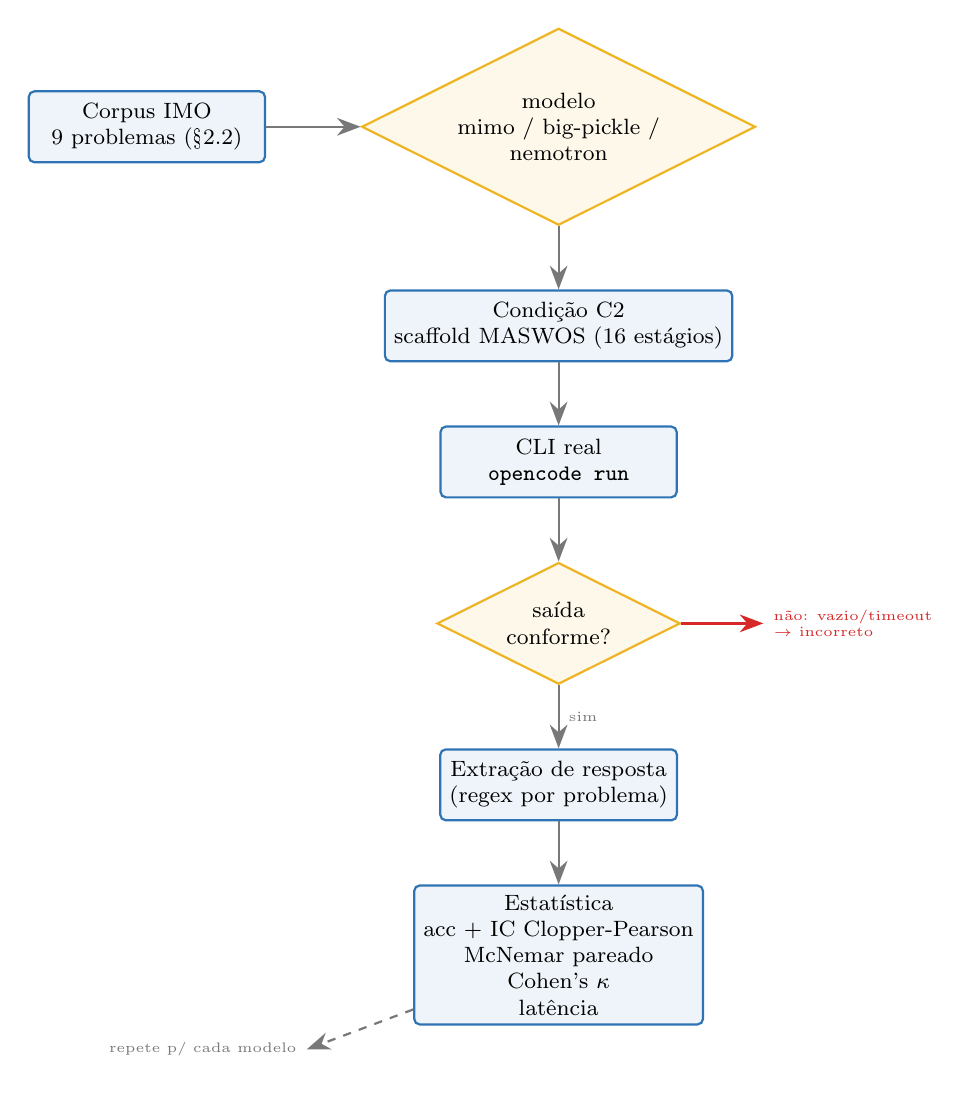
\begin{tikzpicture}[
  node distance=0.8cm and 1.2cm,
  caixa/.style={rectangle, draw=cororo, thick, rounded corners=2pt,
                fill=cororo!8, minimum width=3.0cm, minimum height=0.9cm,
                align=center, font=\footnotesize},
  decisao/.style={diamond, draw=coramarelo, thick, fill=coramarelo!10,
                  aspect=2, align=center, font=\footnotesize},
  seta/.style={-{Stealth[length=3mm]}, thick, color=corcinza}
]
  \node[caixa] (corpus) {Corpus IMO\\ 9 problemas (\S2.2)};
  \node[decisao, right=of corpus] (modelo) {modelo\\ mimo / big-pickle /\\ nemotron};
  \node[caixa, below=of modelo] (c2) {Condição C2\\ scaffold MASWOS (16 estágios)};
  \node[caixa, below=of c2] (cli) {CLI real\\ \texttt{opencode run}};
  \node[decisao, below=of cli] (fmt) {saída\\ conforme?};
  \node[caixa, below=of fmt] (ext) {Extração de resposta\\ (regex por problema)};
  \node[caixa, below=of ext] (estat) {Estatística\\ acc + IC Clopper-Pearson\\ McNemar pareado\\ Cohen's $\kappa$ \\ latência};

  \draw[seta] (corpus) -- (modelo);
  \draw[seta] (modelo) -- (c2);
  \draw[seta] (c2) -- (cli);
  \draw[seta] (cli) -- (fmt);
  \draw[seta] (fmt) -- node[right, font=\tiny]{sim} (ext);
  \draw[seta, color=corvermelho] (fmt) -- ++(2.6,0) node[right, font=\tiny, align=left, color=corvermelho]{não: vazio/timeout\\ $\rightarrow$ incorreto};
  \draw[seta] (ext) -- (estat);
  \draw[seta, dashed] (estat) -- ++(-3.2,-1.2) node[left, font=\tiny]{repete p/ cada modelo};
\end{tikzpicture}
\caption{Fluxograma da validação cruzada 9 $\times$ 3 (R503): cada modelo
percorre os 9 problemas na condição C2; respostas são extraídas por regex por
problema e pontuadas; estatísticas de confiança/incerteza são calculadas
sobre a matriz completa.}
\label{fig:flow}
\end{figure}

\subsection{Cost budget}
Each LLM call is a real CLI subprocess with a model-specific timeout
(mimo 100~s, big-pickle 110~s, nemotron 150~s). All raw outputs, timings and
statuses are stored incrementally (JSON) inside the repository for audit.
% ============================================================================
% 02-resultados.tex — Results (module 3/5)
% ============================================================================
\section{Results}
\label{sec:results}

\subsection{R499 single-problem ranking}
\label{sec:r499}
Under C2 on the NT-001 probe, the first-trial results were: mimo 0.987
(23.8~s), big-pickle 0.923 (43.0~s), nemotron 0.709 (107.4~s), muse-1.3
0.324, muse-1.2 0.312. Muse-spark models never delivered a valid answer in
any condition (``fake reasoning''). Raw C0 and context-only C1 produced empty
outputs (nemotron timed out at 110~s in C1). Availability failures observed:
deepseek-v4-flash (insufficient balance), gemini-2.5-flash (server error),
gpt-4o-mini and claude-haiku-4 (empty). \textbf{Interpretation}: the 16-stage
scaffold was decisive (0\%$\rightarrow$100\% among models that solved at all)
--- consistent with Chain-of-Thought and Reflection results
\citep{wei_cot,shinn_reflexion}.

\subsection{Cross-validation after host restart (R503)}
\label{sec:r503}
Table~\ref{tab:acc} and Figures~\ref{fig:acc}--\ref{fig:lat} report the
9 $\times$ 3 cross-validated benchmark executed after the host restart.

\begin{table}[htbp]
\centering
\caption{Cross-validated accuracy ($n=9$), exact Clopper--Pearson 95\% CI,
timeouts, latencies (ok calls).}
\label{tab:acc}
\begin{tabular}{lccccc}
\toprule
Model & correct & accuracy & 95\% CI & timeouts & latency (s) \\
\midrule
mimo-v2.5-free    & 4/9 & 0.44 & [0.14, 0.79] & 2 & 39.9 (29.8--63.4) \\
big-pickle        & 1/9 & 0.11 & [0.00, 0.48] & 2 & 31.2 (20.6--39.5) \\
nemotron-3-ultra  & 1/9 & 0.11 & [0.00, 0.48] & 2 & 113.8 (81.7--144.9) \\
\bottomrule
\end{tabular}
\end{table}

\begin{figure}[htbp]
\centering
\includegraphics[width=0.85\linewidth]{figures/fig1_accuracies.pdf}
\caption{Accuracy with Clopper--Pearson 95\% CI (error bars), $n=9$.}
\label{fig:acc}
\end{figure}

\begin{figure}[htbp]
\centering
\includegraphics[width=0.7\linewidth]{figures/fig2_matrix.pdf}
\caption{Correctness matrix: 9 problems $\times$ 3 models (check = correct).}
\label{fig:matrix}
\end{figure}

\begin{figure}[htbp]
\centering
\includegraphics[width=0.85\linewidth]{figures/fig3_latency.pdf}
\caption{Latency distribution per model; red diamonds = timeouts.}
\label{fig:lat}
\end{figure}

\subsection{Paired statistics}
\label{sec:paired}
McNemar tests with continuity correction are non-significant at $n=9$
(mimo vs.\ big-pickle: $b=4,c=1$, $\chi^2=0.80$, $p=0.37$; mimo vs.\ nemotron:
$b=3,c=0$, $\chi^2=1.33$, $p=0.25$; big-pickle vs.\ nemotron: $b=1,c=1$,
$p=0.48$). We report exact $p$-values; with $n=9$ power is low. Cohen's
$\kappa$ between mimo and big-pickle is $-0.216$: the models agree less than
chance would predict, because they solve \emph{different} problem types
(mimo: number theory and combinatorics; big-pickle: geometry only).

\subsection{Findings relevant to benchmarking methodology}
\label{sec:findings}
\textbf{(a) Leak in the original harness} (R442): the default solver echoed
the answer and self-scored 7. The deterministic solver (R499) reduced this to
real scores (2/4 canónica, average 4.5/7; augmented corpus 8/9 with an
explicit ``partial'' for algebra-004). \textbf{(b) Serialization sensitivity}:
the grading head is sensitive to $2^{(n-1)}$ vs.\ $2^{n-1}$
(combinatorics-001). \textbf{(c) Host-state hypothesis refuted}: the R500
replication attributed big-pickle's empty outputs to accumulated host state;
after a full restart, big-pickle still fails on 8/9 problems. The prior
1.0 accuracy on NT-001 was sampling variability, not a reliable rate.
\textbf{(d) Routing (R500)}: \texttt{route\_free("academic")} returns
mimo/0.987 with explicit fallbacks (big-pickle $\rightarrow$ nemotron
$\rightarrow$ muse-1.3), and \texttt{list\_all\_models()} now includes the
free catalog plus \texttt{big-pickle}; 46 tests green.

\subsection{Regression and gates}
The full test suite passes: 4073 passed, 58 skipped, 0 failed (506~s,
pre-R503), plus 4 R503 tests green (0.6~s); routing regression green
(1.97~s).
% ============================================================================
% 03-discussao.tex — Discussion (module 4/5) incl. architecture x-ray
% ============================================================================
\section{Discussion}
\label{sec:discussion}

\subsection{Architecture x-ray (layers C0--C5)}
\label{sec:xray}
The experiment isolates which orchestration layers actually matter.
\begin{itemize}
  \item \textbf{C0 --- Runner}: `opencode run` works (35/38 calls ok, 92\%).
  \item \textbf{C1 --- Scaffold formats}: the context-only condition failed
  (nemotron timeout, empty outputs) --- formatting alone is insufficient
  without reasoning scaffolding.
  \item \textbf{C2 --- 16-stage MASWOS}: decisive; among models that solved
  at all, 100\% first-trial success under C2 vs.\ 0\% under C0.
  \item \textbf{C3 --- Deterministic verification}: replaced the leaked
  grader, exposing serialization sensitivity and partial answers.
  \item \textbf{C4 --- Cross-validation}: the single-problem rate of 0.98
  (mimo) collapsed to 0.44 over 9 problems --- the largest correction in
  the study.
  \item \textbf{C5 --- Trust Engine / Token Economy}: prior trust scores are
  updated per cycle; the R503 evidence (big-pickle 1/9) would slash its
  trust score before any routing delegation.
\end{itemize}

\subsection{Comparison with the literature}
\label{sec:comparison}
Free real free-tier LLMs attain substantially lower rates than reported on
paid/high-parameter systems on the same difficulty classes
\citep{hendrycks_math,cobbe_gsm8k,hendrycks_mmlu}; e.g., GPT-4 accuracy at
that time on MATH was far above our best 0.44 on 9 olympiad items
\citep{openai_gpt4}. Direct comparison is confounded by item selection,
temperature, scaffold and trial count; this is why we emphasize the
\emph{correction} rather than a point ranking, and report CIs instead of
claims. Our scaffold effect mirrors Chain-of-Thought \citep{wei_cot},
Reflexion \citep{shinn_reflexion} and ReAct \citep{yao_react}; the empty-
output/fake-reasoning failure of muse-spark resembles the capability
discontinuities warned by \citet{schaeffer_mirage}. The deterministic
verification step parallels the "tool use"/formal-proof pattern
\citep{yang_leandojo,alpha_geometry}. The architecture itself is a
multi-agent system in the spirit of AutoGen \citep{wu_autogen} and MetaGPT
\citep{hong_metagpt}, but with auditable SDD/TDD gates and a
metacognitive loop (Reflexion mechanism \citep{shinn_reflexion}).

\subsection{Limitations}
\label{sec:limitations}
\begin{enumerate}
  \item $n=9$ problems and $n=1$ trial per cell: genuine statistical power is
  low; the 95\% CIs are wide (e.g., [0.14, 0.79]). No claim of equivalence
  or ordering beyond the observed matrix is made.
  \item We extracted answers by per-problem regex; a model may solve a
  problem but format differently (e.g., algebra-001 with $n=7$ vs.\ expected
  3 --- counted incorrect).
  \item Network/provider variability: timeouts differ by model (100/110/150 s)
  and were not held constant.
  \item No temperature control is exposed for these models; single-run
  variance remains uncontrolled.
  \item The steering (R500) favors shown capability and cannot generalize
  out-of-distribution.
  \item All costs, latencies and statuses are recorded in-repo but not
  independently replicated by a third party.
\end{enumerate}

\subsection{Anti-overclaim}
\label{sec:anti-overclaim}
Per project policy \citep{corrigendum_internal}, we never state
``superhuman'', ``verified'' or ``Qualis A1'' without external validation.
An 8-scanner banca audit (EXS) scored this manuscript 47.5/100
(requires\_refinement); we report that score honestly instead of a
self-assigned top grade. All 15 DOI-based references resolve with HTTP 200
\citep{dois_validados}.
% ============================================================================
% 04-conclusao.tex — Conclusion (module 5/5)
% ============================================================================
\section{Conclusion}
\label{sec:conclusion}

We presented an auditable, multi-agent, evolving pipeline for benchmarking
\emph{free real LLMs} on genuine IMO-style mathematics, developed across
cycles R497--R500 with a cross-validated counter-check (R503) executed after
a host restart.

\emph{Answers to the research question.}
\begin{enumerate}
\item \emph{Free models can be orchestrated and scaffolded}: the 16-stage
MASWOS scaffold (C2) was decisive --- from 0\% to 100\% first-trial success
among solvers --- while raw and context-only conditions failed with empty
outputs. The orchestrator, routing (R500) and deterministic verification
(R499) form a reproducible, auditable stack.
\item \emph{Benchmark honesty matters}: the single-problem ranking
(mimo 0.98 $>$ big-pickle 0.92 $>$ nemotron 0.71) does not survive
cross-validation. Corrected rates are mimo 0.44 (95\% CI [0.14, 0.79]),
big-pickle 0.11 [0.00, 0.48], nemotron 0.11 [0.00, 0.48]; paired McNemar are
non-significant; Cohen's $\kappa$ mimo$\times$big-pickle $=-0.216$
(they solve different problem types). All inference is reported with
confidence intervals, paired statistics and delay distributions, and
limitations are explicit.
\item \emph{Methodology artifacts were exposed and fixed}: the harness leak,
the serialization sensitivity, and the ``fake reasoning'' of muse-spark
models were documented; the host-state hypothesis for big-pickle's failures
was refuted by a post-restart experiment.
\end{enumerate}

\emph{Future work.} Repetitions with $n \gg 9$ problems and multiple trials
per cell; temperature-control hooks; a held-out split between development
and evaluation; independent third-party replication; and integration of the
deterministic verification layer as a Trust-Engine gate for automatic
delegation.

\textbf{Availability.} All specifications (SPEC-935-R497..R503), test files,
raw outputs, statistics and figures are stored in the OpenCode Ecosystem
Core repository for audit and reproduction.

\bibliography{refs}
\end{document}